% !TEX root = Principal.tex

% Desenvolvido por: Prof. Dr. David Buzatto
% Adaptado por: Prof. Dr. Fernando Carvalho
% Atualizado por: Kevin Siqueira Perdomo, graduando em Engenharia da Computação
%
% Baseado na documentação do abntex2 e nos modelos em
% Microsoft Word propostos pela Profa. Dra. Rosana F. L. Rodrigues
% e pela bibliotecária M.Sc. Maria Carolina Gonçalves do câmpus
% São João da Boa Vista do IFSP.
%
% Atualizado para seguir as normas ABNT mais recentes:
% - NBR 14724:2024 (Estrutura de trabalhos acadêmicos)
% - NBR 6023:2025 (Elaboração de referências)
% - NBR 10520:2023 (Citações)
%
% Versão 2.0
% Data: 04/09/2025


\documentclass[
	% -- opções da classe memoir --
	12pt,				% tamanho da fonte
	openany,			% capítulos começam em pág ímpar openright (insere página vazia caso preciso)
	oneside,			% para impressão em verso e anverso (twoside). Oposto a oneside 
	a4paper,			% tamanho do papel. 
	normalfigtabnum,
	pnumromarab,
	% -- opções da classe abntex2 --
	chapter=TITLE,		% títulos de capítulos convertidos em letras maiúsculas
	section=TITLE,		% títulos de seções convertidos em letras maiúsculas
	%subsection=TITLE,	% títulos de subseções convertidos em letras maiúsculas
	%subsubsection=TITLE,% títulos de subsubseções convertidos em letras maiúsculas
	% -- opções do pacote babel --
	english,			% idioma adicional para hifenização
	french,				% idioma adicional para hifenização
	spanish,			% idioma adicional para hifenização
	brazil,				% o último idioma é o principal do documento
]{abntex2}

% \usepackage{blindtext, showframe}

% \usepackage[a4paper,showframe,
% top    = 2.75cm,
% bottom = 2.50cm,
% left   = 3.00cm,
% right  = 2.50cm]{geometry}


%%%%%%%%%%%%%%%%%%%%%%%%%%%%%%%%%%%%%%%%%%%%%%%%%%%%%%%%%%%%


\newenvironment{conditions}[1][onde:]
  {\noindent
	#1
	
	\indent
	\begin{tabular}[t]{>{$}l<{$} @{${} \> \> {}$} l}}
	{\end{tabular}\\[\belowdisplayskip]}


% --- Controla a geração de listas de siglas, símbolos e glossário
% \RequirePackage[style=long]{glossaries}
% ,long,numberlist


\usepackage[acronyms,symbols]{glossaries}
\setacronymstyle{long-short}

\makenoidxglossaries


%Definição das listas de glossários e parâmertos para compilação.
%-------------------------------------------------------
\newglossary{verbetes}{verbetes}{vrl}{verbetes}
\newglossary{siglas}{siglas}{sgl}{siglas}
\newglossary{simbolos}{simbolos}{sbl}{simbolos}


%Definição dos comandos para exibição das listas individuais.
%-----------------------------------------------------------
\newcommand{\listarsiglas}{\printglossary[type=siglas, title=\listadesiglasname, nonumberlist=true]}
\newcommand{\listarsimbolos}{\printglossary[type=simbolos, title=\listadesimbolosname, nonumberlist=true]}
\newcommand{\listarverbetes}{\printglossary[type=verbetes]}

%Definição dos Comandos para inclusão no texto das siglas.

\newcommand{\verbete}[3]{
	\newglossaryentry{glossary}{name=#1, description={#2}, plural={#3}, type=verbetes}
	\gls{#1}
}

\newcommand{\sigla}[2]{
	\newacronym[type=siglas]{#1}{#1}{#2}
	\gls{#1}
}

\newcommand{\simbolo}[3]{
	\newglossaryentry{#1}{type=simbolos, name=#3, text=#3, description=#2,symbol=#3, sort=def}
	\gls{#1}
}

%%%%%%%%%%%%%%%%%%%%%%%%%%%%%%%%%%%%%%%%%%%%%%%%%%%%%%%%%%%%

\RequirePackage{bookmark}   			



% ---------------------------------------------------------------------------------
%                                   PACOTES
% ---------------------------------------------------------------------------------


% ---
% Pacotes básicos 
% ---

\usepackage{cmap}
\usepackage{lmodern}

\usepackage{amsmath}
\usepackage{latexsym}
\usepackage{amsfonts}
\usepackage[normalem]{ulem}
\usepackage{array}
\usepackage{amssymb}
\usepackage{graphicx}

% \usepackage[backend=bibtex,
% style=authoryear,
% natbib=true,
% sorting=none,
% isbn=false,
% doi=false,
% url=false,

\usepackage{subfig}
\usepackage{wrapfig}
\usepackage{wasysym}
\usepackage{enumitem}
\usepackage{adjustbox}
\usepackage{ragged2e}
\usepackage[svgnames,table]{xcolor}
\usepackage{tikz}
\usetikzlibrary{intersections}
\usetikzlibrary{shapes,arrows,chains}
\tikzstyle{line}=[draw] % here
\usepackage{longtable}
\usepackage{changepage}
\usepackage{setspace}
\usepackage{hhline}
\usepackage{multicol}
\usepackage{tabto}
\usepackage{multirow}
\usepackage{makecell}
\usepackage{fancyhdr}



\usepackage{lmodern}			% Usa a fonte Latin Modern			
\usepackage[T1]{fontenc}		% Selecao de codigos de fonte.
\usepackage[utf8]{inputenc}		% Codificacao do documento (conversão automática dos acentos)
\usepackage{lastpage}			% Usado pela Ficha catalográfica
\usepackage{indentfirst}		% Indenta o primeiro parágrafo de cada seção.
\usepackage{xcolor,colortbl}	% Controle das cores
\usepackage{graphicx}			% Inclusão de gráficos
\usepackage{microtype} 			% para melhorias de justificação
\usepackage{hyperref}
\usepackage{subfig}
\usepackage{epigraph}
\usepackage{url}
\usepackage{placeins}
\usepackage{multirow}
\usepackage[figuresright]{rotating}
\usepackage{chemfig}
\usepackage{amsmath}
\usepackage{amssymb}
\usepackage{enumitem}
\usepackage{bigints}
\usepackage{listings}
\usepackage{etoolbox}
\usepackage[final]{pdfpages}
\usepackage{bigstrut}
\usepackage{makeidx}
\usepackage{float}
\usepackage{booktabs}
\usepackage{siunitx}			% para unidades no SI
% ---



% ---
% Pacotes adicionais, usados apenas no âmbito do Modelo Canônico do abnteX2
% ---
\usepackage{lipsum}				% para geração de dummy text
% ---

% ---
% Pacotes de citações
% ---
% \usepackage[brazilian,hyperpageref]{backref}	 % Paginas com as citações na bibl
% \usepackage[alf,abnt-emphasize=bf]{abntex2cite}  % Citações padrão ABNT

% Citações conforme NBR 10520:2023 e referências conforme NBR 6023:2025
% Configuração: et al. para mais de 3 autores, formatação ABNT atualizada
% O abntex2-alf ordena automaticamente por sobrenome do primeiro autor
\usepackage[alf,abnt-emphasize=bf,abnt-full-initials=yes,abnt-etal-cite=3,abnt-etal-list=3,abnt-thesis-year=final,abnt-url-package=url]{abntex2cite}  


% ---------------------------------------------------------------------------------
%                          CONFIGURAÇÕES DOS PACOTES
% ---------------------------------------------------------------------------------

% ---
% Configurações do pacote backref
%
% Para desativar, tire o comentário de \begin{comment} e \end{comment} 
% das próximas linhas e comente a linha \usepackage[brazilian,hyperpageref]{backref}
% acima.
% ---

% \newcommand{\imprimirdata}{\data}


\begin{comment}
% ---
% Configurações do pacote backref
% Usado sem a opção hyperpageref de backref
\renewcommand{\backrefpagesname}{Citado na(s) página(s):~}
% Texto padrão antes do número das páginas
\renewcommand{\backref}{}
% Define os textos da citação
\renewcommand*{\backrefalt}[4]{
	\ifcase #1 %
	Nenhuma citação no texto.%
	\or
	Citado na página #2.%
	\else
	Citado #1 vezes nas páginas #2.%
	\fi}%
% ---
\end{comment}


% listagens
\definecolor{corComentario}{RGB}{150,150,150}
\definecolor{corString}{RGB}{206,123,0}
\definecolor{corPalavraChave}{RGB}{0,0,230}

\lstset{
	numbers=left,
	stepnumber=1,
	firstnumber=1,
	numberstyle=\footnotesize,
	extendedchars=true,
	breaklines=true,
	lineskip=0pt,
	frame=tb,
	basicstyle=\ttfamily\footnotesize,
	showstringspaces=false,
	stringstyle=\color{corString},
	commentstyle=\color{corComentario},
	keywordstyle=\color{corPalavraChave}
}

\newcommand{\graficoname}{Gráfico}
\newcommand{\graficorefname}{Gráfico}
\newcommand{\listofgraficosname}{Lista de gráficos}





% \newcolumntype{Y}{>{\centering\arraybackslash}X}

\newcommand{\ano}[1]{\def \oano {#1}}
\newcommand{\imprimirano}{\oano}

\newcommand{\mes}[1]{\def \omes {#1}}
\newcommand{\imprimirmes}{\omes}

\newcommand{\dia}[1]{\def \odia {#1}}
\newcommand{\imprimirdia}{\odia}

% \newcommand{\subtitulo}[1]{\def \osubtitulo {#1}}
% \newcommand{\imprimirsubtitulo}{\osubtitulo}

\newcommand{\area}[1]{\def \aarea {#1}}
\newcommand{\imprimirarea}{\aarea}

\newcommand{\disciplina}[1]{\def \adisciplina {#1}}
\newcommand{\imprimirdisciplina}{\adisciplina}

% \renewcommand{\coorientador}[1]{\def \ocoorientador {#1}}
% \renewcommand{\imprimircoorientador}{\ocoorientador}

\newcommand{\grau}[1]{\def \ograu {#1}}
\newcommand{\imprimirgrau}{\ograu}

\newcommand{\curso}[1]{\def \ocurso {#1}}
\newcommand{\imprimircurso}{\ocurso}

\newcommand{\campus}[1]{\def \ocampus {#1}}
\newcommand{\imprimircampus}{\ocampus}

\newcommand{\instituicaoOrientador}[1]{\def \aInstituicaoOrientador {#1}}
\newcommand{\imprimirInstituicaoOrientador}{\aInstituicaoOrientador}

\newcommand{\instituicaoCoorientador}[1]{\def \aInstituicaoCoorientador {#1}}
\newcommand{\imprimirInstituicaoCoorientador}{\aInstituicaoCoorientador}

\newcommand{\instituicaoProfBancaA}[1]{\def \aInstituicaoProfBancaA {#1}}
\newcommand{\imprimirInstituicaoProfBancaA}{\aInstituicaoProfBancaA}

\newcommand{\instituicaoProfBancaB}[1]{\def \aInstituicaoProfBancaB {#1}}
\newcommand{\imprimirInstituicaoProfBancaB}{\aInstituicaoProfBancaB}

\providecommand{\imprimirProfBancaARotulo}{}
\providecommand{\imprimirProfBancaAnome}{}
\newcommand{\ProfBancaA}[2][\ProfBancaAname]%
  {\renewcommand{\imprimirProfBancaARotulo}{#1}%
   \renewcommand{\imprimirProfBancaAnome}{#2}}


\providecommand{\imprimirProfBancaBRotulo}{}
\providecommand{\imprimirProfBancaBnome}{}
\newcommand{\ProfBancaB}[2][\ProfBancaBname]%
  {\renewcommand{\imprimirProfBancaBRotulo}{#1}%
   \renewcommand{\imprimirProfBancaBnome}{#2}}



% Área de Concentração: \imprimirarea}
% ---


% ---
% Configurações de aparência do PDF final
% ---

% alterando o aspecto da cor azul
\definecolor{blue}{RGB}{41,5,195}

% informações do PDF
\makeatletter
\hypersetup{
	%pagebackref=true,
	pdftitle={\@title}, 
	pdfauthor={\@author},
	pdfsubject={\imprimirpreambulo},
	pdfcreator={\@author},
	pdfkeywords={Palavra chave 1}{Palavra chave 2}{Palavra chave 3}{Palavra chave n}, 
	colorlinks=true,       		% false: boxed links; true: colored links
	linkcolor=blue,          	% color of internal links
	citecolor=blue,       		% color of links to bibliography
	filecolor=black,      		% color of file links
	urlcolor=blue,
	bookmarksdepth=4
}
\makeatother
% --- 


% ---
% Comandos do autor
% ---

% comando para inserir autor e ano
\newcommand{\citeauthorandyear}[1]{\citeauthoronline{#1} (\citeyear{#1})}

% --- 
% Espaçamentos entre linhas e parágrafos 
% --- 

% O tamanho do parágrafo é dado por:
\setlength{\parindent}{1.3cm}

% Controle do espaçamento entre um parágrafo e outro:
\setlength{\parskip}{0.2cm}  % tente também \onelineskip

\glsaddall

% ---
% compila os glossários e listas
%\makeglossaries

% ---
% compila o indice
% ---
\makeindex
% ---
%---


%%%%%%%%%%%%%%%%%%%%%%%%%%%%%%%%%%%%%%%%%%%%

% para o pacote "Lst Listing"

\newcommand{\source}[1]{\caption*{Fonte: {#1}}}

% Altera o nome padrão do rótulo usado no comando \autoref{}
\renewcommand{\lstlistingname}{Código}

% Altera o rótulo a ser usando no elemento pré-textual "Lista de código"
\renewcommand{\lstlistlistingname}{Lista de códigos}

%% Configuração para o ambiente de código (algorítmos)
\lstset{
%   numbers=left,
%   inputencoding=latin1,
%   basicstyle=\footnotesize\ttfamily,
%   keywordstyle=\color{blue},         
%   breaklines=true, 
%   showtabs=false,
%   showstringspaces=false,
%   numberstyle=\tiny\color{mygray}
   basicstyle=\fontsize{9}{11}\selectfont\ttfamily
}
%% 
%% exemplo da página https://latex.org/forum/viewtopic.php?t=24038
%%

\newglossaryentry{K-I}{type=symbols,name=$K_{I}$,
	symbol={$K_{I}$},
	description={fator de intensificador, modo I de abertura de trinca}}


\newglossaryentry{K-IC}{type=symbols,name=$K_{IC}$,
	symbol={$K_{IC}$},
	description={tenacidade à fratura do modo I de abertura de trinca}}

% Peterson - Pilkey (pag 2)
\newglossaryentry{sigma-max}{type=symbols,name={$\sigma_{max}$},
	symbol={$\sigma_{max}$},
	description={tensão normal máxima}}


\newglossaryentry{a}{type=symbols,name=$a$,
	symbol={$a$},
	description={profundidade da trinca}}


\newglossaryentry{rho}{type=symbols,name={$\rho$},
	symbol={$\rho$},
	description={raio na ponta do entalhe}}

% Tanaka
\newglossaryentry{h}{type=symbols,name={$h$},
	symbol={$h$},
	description={altura do corpo de prova}}


% tanaka 2003
\newglossaryentry{F-a-h}{type=symbols,name={$F(a/h)$},
	symbol={$F(a/h)$},
	description={fator de ajuste de geometria}}


\newglossaryentry{a-0}{type=symbols,name={$a_{0}$},
	symbol={$a_{0}$},
	description={profundidade inicial do entalhe}}


\newglossaryentry{rpm}{type=acronym,name={RPM},
	description={rotações por minuto}}

\newglossaryentry{sms}{type=acronym,name={SMS},
	description={mensagens de texto}}




% ---------------------------------------------------------------------
% Informações de dados para CAPA, FOLHA DE ROSTO e FOLHA DE ASSINATURAS
% ---------------------------------------------------------------------

% ---------------------------------------------------------------------
% Alterar os dados abaixo com os seus dados
% ---------------------------------------------------------------------

\curso{Bacharelado em Engenharia da Computação}
\grau{Bacharel em  em Engenharia da Computação} 
\titulo{Uma Proposta de Padronização de Modelo para a Criação de TCCs dos Cursos de Computação do Instituto Federal Fluminense}
\tipotrabalho{Trabalho de Conclusão}
\area{Tecnologia da Informação}

\autor{Nome do Primeiro Aluno \\ Nome do Segundo Aluno}
\orientador{Prof. D.Sc. 
Nome do Professor Orientador}
\instituicaoOrientador{Instituto Federal Fluminense (IFF)}

% caso não haja coorientador, comente a linha abaixo
\coorientador{Profa. M.Sc. 
Nome da Professora Coorientadora}
\instituicaoCoorientador{Instituto Federal Fluminense (IFF)}

\ProfBancaA{Prof. D.Sc. 
Nome do Professor Membro da Banca}
\instituicaoProfBancaA{Instituto Federal Fluminense (IFF)}

\ProfBancaB{Prof. D.Sc.
Nome do Outro Professor Membro da Banca}
\instituicaoProfBancaB{Instituto Federal Fluminense (IFF)}

\local{Campos dos Goytacazes-RJ}
\dia{29}
\mes{março}
\ano{2019}
\data{Março de \imprimirano}

\instituicao{Instituto Federal de Educação, Ciência e Tecnologia Fluminense}
\campus{Campos-Centro}

\preambulo{\imprimirtipotrabalho\ apresentado ao curso \imprimircurso~ do \imprimirinstituicao, como parte dos requisitos para a obtenção do título de \imprimirgrau.}

% ---------------------------------------------------------------------------------
%                                   INÍCIO DO DOCUMENTO
% ---------------------------------------------------------------------------------

\begin{document}

\pretextual

\imprimircapa 

% \imprimirfolhaderosto

% 
% ---
% Inserir folha de aprovação
% ---

% Isto é um exemplo de Folha de aprovação, elemento obrigatório da NBR
% 14724/2011 (seção 4.2.1.3). Você pode utilizar este modelo até a aprovação
% do trabalho. Após isso, substitua todo o conteúdo deste arquivo por uma
% imagem da página assinada pela banca com o comando abaixo:
%
\begin{folhadeaprovacao}
	\includepdf{pre/FolhaAprovacaoAssinadaEscaneada}
\end{folhadeaprovacao}

%
\begin{folhadeaprovacao}

\setlength{\ABNTEXsignwidth}{14cm}

    \begin{center}
    {\ABNTEXchapterfont\large\imprimirautor}

    \vspace*{\fill}\vspace*{\fill}
    {\ABNTEXchapterfont\bfseries\Large\imprimirtitulo}
    \vspace*{\fill}
    
    \hspace{.45\textwidth}
    \begin{minipage}{.5\textwidth}
        \imprimirpreambulo
    \end{minipage}%
    \vspace*{\fill}
   
   \end{center}
 
 
   \begin{center}
    \imprimirlocal, \imprimirdia ~de \imprimirmes ~de \imprimirano.
   \end{center}
   
   % Instituto Federal Fluminense (IFF)
   \assinatura{\textbf{\imprimirProfBancaARotulo \imprimirProfBancaAnome} \\%
   \imprimirInstituicaoProfBancaA}
   
   \assinatura{\textbf{\imprimirProfBancaBRotulo \imprimirProfBancaBnome} \\%
   \imprimirInstituicaoProfBancaB}
   
   \assinatura{\textbf{\imprimirorientadorrotulo \imprimirorientador} \\%
   \imprimirInstituicaoOrientador}
   
   \assinatura{\textbf{\imprimircoorientadorrotulo \imprimircoorientador} \\%
   \imprimirInstituicaoCoorientador}

   \begin{center}
    \vspace*{0.5cm}
    {\large\imprimirlocal}
    \par
    {\large\imprimirdata}
    \vspace*{1cm}
  \end{center}
  
\end{folhadeaprovacao}
% ---


% 
\begin{agradecimentos}

Acima de tudo, agradecemos a Deus pelo dom da vida e pela conclusão do projeto.

Dedicamos este trabalho a nossa família, amigos, ao nosso professor...

\end{agradecimentos}




% \begin{resumo}

% O comando lipsum abaixo é um gerador automático de texto.
% Substitua-o pelo texto do seu resumo.
% Lembre-se: Um resumo deve ser um parágrafo único que apresente os seguintes tópicos:

% Contexto;
% Problema;
% Objetivo;
% Justificativa;
% Metodologia;
% Resultado;
% Conclusão.

\lipsum*[10-12]

\textbf{Palavras-chaves: } Curabitur, Malesuada, MassaAndroid, Aliquam.  

\end{resumo}




% \begin{resumo}[Abstract]
 \begin{otherlanguage*}{english}

% O comando lipsum abaixo é um gerador automático de texto, e deve ser substituído pelo seu abstract, isto é, o seu resumo traduzido para a lingua inglesa.

\lipsum*[10-12]

\textbf{Keywords: } Curabitur, Malesuada, MassaAndroid, Aliquam. 

 \end{otherlanguage*}
\end{resumo}



% não é necessário alterar este arquivo

\listoffigures*
\clearpage


% não é necessário alterar este arquivo

\listofquadros
\clearpage


% não é necessário alterar este arquivo

\listoftables*
\clearpage


% não é necessário alterar este arquivo

\listofcodigos*
\clearpage


% %\listarsiglas

% \begin{siglas}
% \item[API] Application Programming Interface
% \item[ABRELPE] Associação Brasileira de Empresas de Limpeza Pública e Resíduos Especiais
% \item[APK] Android Package
% \item[APP] Application
% \item[BaaS] Backend as a Service
% \item[CASE] Computer-Aided Software Engineering
% \item[GPS] Global Positioning System
% \item[IDE] Integrated Development Environment
% \item[IPEA] Instituto de Pesquisa Econômica Aplicada
% \item[JSON] JavaScript Object Notation
% \item[JVM] Java Virtual Machine
% \item[MNCR] Movimento Nacional dos Catadores de Materiais Recicláveis
% \item[NoSQL] Not only SQL
% \item[OHA] Open Handset  Alliance
% \item[ONU] Organização das Nações Unidas
% \item[PNRS] Política Nacional de Resíduos Sólidos 
% \item[SDK] Software Development Kit
% \item[SIG] Sistemas de Informação Geográfica
% \item[WWW]  Apple Worldwide Developers Conference
% \end{siglas}

% \printglossaries
\makeglossaries
\printglossary

% \begin{verbatim}
% API \tab Application Programming Interface\\
% APK \tab Android Package\\
% APP \tab Application\\
% BaaS \tab Backend as a Service\\
% GPS\tab Global Positioning System\\
% IDE \tab Integrated Development Environment\\
% JSON \tab  JavaScript Object Notation\\
% JVM \tab   Java Virtual Machine\\
% NoSQl \tab Not Only SQL\\
% SDK \tab  Software Development Kit
% \end{verbatim}


\setglossarypreamble[acronym]{%
	\glsresetentrycounter
}
\setglossarystyle{long3col}
\printnoidxglossary[type=acronym]

\clearpage


% 
\setglossarypreamble[symbols]{%
	\glsresetentrycounter
}

\setglossarystyle{long3col}

\printnoidxglossary[type=symbols]

\clearpage



 %%%%%%%%%%%%  This Produces Table Of Contents %%%%%%%%%%%%%%
\vspace{\baselineskip}
\setlength{\parskip}{0.0pt}

\begin{Center}
\end{Center}\par

\vspace{\baselineskip}
\setlength{\parskip}{9.96pt}

\tableofcontents
\addcontentsline{toc}{chapter}{Contents}

\clearpage
 %%%%%%%%%%%%  Starting New Page here %%%%%%%%%%%%%%


\textual

\chapter{INTRODUÇÃO}
\label{cap:introducao}

\section{Problema e Contexto}

Nos últimos anos, a combinação entre o avanço do poder computacional e o desenvolvimento de algoritmos mais sofisticados tem impulsionado significativamente a área de visão computacional. Essa área da inteligência artificial tem se mostrado essencial em diversas aplicações, desde sistemas de segurança e monitoramento, até diagnósticos médicos e veículos autônomos \cite{szeliski2022computer}. Nesse cenário, o reconhecimento de padrões e a detecção de objetos se tornaram tarefas cada vez mais precisas e eficientes, aproximando as capacidades das máquinas da percepção humana.

O reconhecimento de objetos em imagens é uma atividade simples para humanos quando possuem expertise no assunto e está se tornando cada vez mais acessível aos computadores, devido aos avanços em estudos de visão computacional que utilizam redes neurais de aprendizagem profunda \cite{goodfellow2016deep}. Segundo \citeonline{haykin2009neural}, a aprendizagem profunda é "uma subárea da aprendizagem de máquina que emprega algoritmos inspirados no funcionamento do cérebro humano, simulando um conjunto de neurônios conectados e organizados em camadas, onde cada camada processa informações e transmite o resultado para a próxima".

Com a popularização de arquiteturas como as Redes Neurais Convolucionais (CNNs), tornou-se possível processar grandes volumes de dados visuais com alta acurácia. Essas redes têm a capacidade de extrair automaticamente características relevantes das imagens, dispensando a necessidade de intervenção manual no processo de extração de atributos \cite{lecun2015deep}. Como resultado, surgem soluções mais robustas e adaptáveis, contribuindo diretamente para a expansão de aplicações baseadas em visão computacional.

\section{Objetivos}

O presente trabalho tem como objetivo comparar o desempenho de diferentes arquiteturas de detecção de objetos YOLO, Faster R-CNN, SSD, EfficientDet e RetinaNet utilizando datasets de referência, como COCO e PASCAL VOC. A análise abrangerá métricas quantitativas de desempenho, como precisão, recall, mean Average Precision (mAP) e tempo de inferência, bem como uma discussão crítica sobre a aplicabilidade de cada modelo em diferentes cenários, visando fornecer subsídios para a escolha do algoritmo mais adequado a cada contexto.

\subsection{Objetivo Geral}

O objetivo geral deste trabalho é realizar uma análise comparativa de diferentes arquiteturas de redes neurais artificiais para a tarefa de detecção de objetos, avaliando seu desempenho em termos de acurácia, velocidade e eficiência computacional.

\subsection{Objetivos Específicos}

Para alcançar o objetivo geral proposto, foram definidos os seguintes objetivos específicos:
\begin{itemize}

\item Realizar uma revisão bibliográfica sobre os principais algoritmos de detecção de objetos baseados em redes neurais convolucionais;

\item Selecionar e implementar os modelos YOLO, Faster R-CNN, SSD, EfficientDet e RetinaNet em ambiente TensorFlow;

\item Preparar e pré-processar datasets públicos (COCO e PASCAL VOC) para treinamento e avaliação;

\item Otimizar os hiperparâmetros de cada modelo para garantir uma comparação justa;

\item Treinar os modelos selecionados e avaliar seu desempenho utilizando métricas padronizadas;

\item Coletar e analisar métricas como mAP (mean Average Precision), precisão, recall e FPS (Frames per Second);

\item Realizar uma análise crítica comparativa dos resultados obtidos, considerando as vantagens e limitações de cada arquitetura.

\end{itemize}

\section{Justificativa}

A evolução das arquiteturas de detecção de objetos, como YOLO, Faster R-CNN, SSD, EfficientDet e RetinaNet, impulsionou significativamente a precisão e a velocidade de sistemas de visão computacional \cite{redmon2016yolo, ren2017faster, liu2016ssd, tan2020efficientdet, lin2020focal}. No entanto, apesar dos avanços, cada modelo apresenta características, vantagens e limitações que podem torná-lo mais adequado para determinados contextos e restrições de hardware.

Como afirmam \citeonline{liu2016ssd}, modelos como o SSD se destacam pela alta velocidade de inferência, enquanto arquiteturas como Faster R-CNN \cite{ren2017faster} priorizam a precisão em detrimento do tempo de processamento. Já o YOLO, segundo \citeonline{redmon2016yolo}, "propõe uma abordagem unificada e em tempo real para a detecção de objetos, transformando o problema em uma única tarefa de regressão".

Nesse sentido, torna-se fundamental compreender, de forma comparativa, o desempenho dessas arquiteturas frente a diferentes bases de dados e condições de inferência. Uma análise comparativa criteriosa permite identificar quais modelos oferecem melhor equilíbrio entre precisão e velocidade, considerando não apenas métricas quantitativas, mas também a complexidade de implementação e a escalabilidade. Essa abordagem auxilia na escolha da solução mais adequada e contribui para o avanço do estado da arte.

\section{Estrutura do Trabalho}

Este trabalho está dividido em sete capítulos. O \autoref{cap:introducao} expõe o contexto do estudo, o problema de pesquisa, as justificativas desta pesquisa e os objetivos a serem atingidos. O \autoref{cap:fundamentacao} apresenta a fundamentação teórica sobre redes neurais convolucionais, algoritmos de detecção de objetos e métricas de avaliação. O \autoref{cap:trabalhos} apresenta uma revisão dos trabalhos relacionados na área de detecção de objetos. O \autoref{cap:metodologia} descreve a metodologia empregada, os datasets utilizados e o ambiente experimental. O \autoref{cap:desenvolvimento} detalha a implementação dos modelos e os procedimentos de treinamento. O \autoref{cap:resultados} apresenta e discute os resultados obtidos na análise comparativa. Finalmente, o \autoref{cap:conclusão} apresenta as conclusões e sugere trabalhos futuros.

\chapter{FUNDAMENTAÇÃO TEÓRICA}
\label{cap:fundamentacao}

\section{Visão Computacional e Aprendizado de Máquina}

\subsection{Fundamentos da Visão Computacional}
% Adicione aqui o conteúdo sobre fundamentos da visão computacional

\subsection{Introdução ao Aprendizado de Máquina e Redes Neurais Profundas}
% Adicione aqui o conteúdo sobre aprendizado de máquina e redes neurais profundas

\section{Redes Neurais Convolucionais (CNNs)}

\subsection{Conceitos Essenciais e Funcionamento das CNNs}
% Adicione aqui o conteúdo sobre CNNs

\section{Principais Arquiteturas de Detecção de Objetos}

\subsection{You Only Look Once (YOLO)}
% Adicione aqui o conteúdo específico sobre YOLO

\subsection{Faster R-CNN}
% Adicione aqui o conteúdo específico sobre Faster R-CNN

\subsection{Single Shot MultiBox Detector (SSD)}
% Adicione aqui o conteúdo específico sobre SSD

\section{TensorFlow}

\subsection{Utilização do Framework no Projeto}
% Adicione aqui o conteúdo sobre como o TensorFlow será utilizado no projeto

\section{Ambiente de Desenvolvimento}

\subsection{Definição do Hardware (Google Colab)}
% Adicione aqui detalhes sobre a configuração do ambiente no Google Colab

\section{Datasets}

\subsection{Seleção e Pré-processamento dos Datasets}
% Adicione aqui detalhes sobre os datasets que serão utilizados e seu pré-processamento

% ============================================================
% CAPÍTULO 3 - TRABALHOS RELACIONADOS
% ============================================================
\chapter{Trabalhos Relacionados}
\label{cap:trabalhos}

A análise comparativa de arquiteturas de redes neurais para tarefas de visão computacional tem
sido um campo fértil de pesquisa, buscando estabelecer os modelos mais eficientes para
diferentes contextos de aplicação. Nesta seção, são apresentados trabalhos que, assim como
este, se dedicaram a comparar o desempenho de diferentes arquiteturas, seja em problemas de
classificação de imagens ou na detecção de objetos. A análise destes estudos é fundamental
para contextualizar a presente pesquisa, identificar as metodologias consolidadas e destacar
as lacunas que este trabalho se propõe a preencher.

% ------------------------------------------------------------
% 3.1 Análise Comparativa de CNNs para Triagem de Lesões de Pele
% ------------------------------------------------------------
\section{Análise Comparativa de CNNs para Triagem de Lesões de Pele}

Em um estudo focado na área médica, \citeonline{santos2019analise} realizou uma análise comparativa
entre as arquiteturas ResNet, VGG e GoogLeNet para a tarefa de triagem e classificação de
lesões de pele. O objetivo era avaliar a viabilidade de utilizar estas redes para apoiar o
diagnóstico médico a partir de um vasto conjunto de dados de 140.446 imagens obtidas em um
cenário real do sistema de saúde.

Após conduzir 42 cenários experimentais, variando arquiteturas, estratégias de inicialização
de pesos e taxas de aprendizado, o autor concluiu que a arquitetura GoogLeNet, com
inicialização randômica dos pesos, apresentou o melhor desempenho. O modelo atingiu 89,72\%
de acurácia para sugestão diagnóstica e 96,03\% para o encaminhamento adequado do paciente.

O trabalho de \citeonline{santos2019analise} é relevante por comparar arquiteturas de base
(\textit{backbones}) que também são utilizadas nos modelos de detecção de objetos, embora seu
foco seja estritamente a classificação.

% ------------------------------------------------------------
% 3.2 Estudo Comparativo de CNNs para Classificação de Imagens
% ------------------------------------------------------------
\section[Estudo Comparativo de CNNs para Classificação de Imagens]{Estudo Comparativo de CNNs para\\Classificação de Imagens}

De forma semelhante, \citeonline{silva2018estudo} conduziu um estudo comparativo direto entre as
arquiteturas VGG-16, ResNet-50 e Inception, aplicando-as a um problema de classificação de
imagens de um domínio específico: a identificação de personagens do desenho ``Os Simpsons''.
O autor buscou avaliar o poder de generalização dessas redes, pré-treinadas com o
\textit{dataset} ImageNet, em um conjunto de dados visualmente distinto.

Utilizando métricas como acurácia e \textit{log loss}, e testando diferentes otimizadores, o
estudo concluiu que a ResNet-50 obteve a maior acurácia (93,4\%), enquanto a Inception
alcançou o menor \textit{log loss} (0.26). Uma das principais constatações foi que a escolha
do otimizador (SGD em vez de RMSprop) foi crucial para o bom desempenho das redes. Este
trabalho corrobora a necessidade de uma análise empírica para determinar a arquitetura mais
adequada para um dado problema de classificação.

% ------------------------------------------------------------
% 3.3 Análise Comparativa de Modelos de Detecção de Objetos
% ------------------------------------------------------------
\section[Análise Comparativa de Modelos de Detecção de Objetos]{Análise Comparativa de Modelos de\\Detecção de Objetos}

Diferentemente dos trabalhos anteriores que focam na classificação,
\citeonline{su2025comparative} apresenta uma análise comparativa que aborda diretamente os três
modelos centrais deste TCC: Faster R-CNN, SSD e YOLO. O autor realiza uma revisão sistemática,
comparando as arquiteturas com base em dados de literatura sobre três eixos principais:
precisão (mAP), velocidade (FPS) e consumo de recursos (GPU VRAM).

A análise de \citeonline{su2025comparative} destaca o claro \textit{trade-off} entre os modelos: a
Faster R-CNN, uma abordagem de dois estágios, alcança alta precisão (73.2\% mAP) sendo ideal
para tarefas que não exigem tempo real, mas consome mais recursos; a YOLO, por sua vez,
prioriza a velocidade (45 FPS), sendo adequada para aplicações em tempo real, ao custo de uma
menor precisão (63.4\% mAP); por fim, a SSD se posiciona como uma solução de equilíbrio entre
velocidade e acurácia. Este artigo fornece um referencial teórico robusto para a comparação
que será realizada de forma prática neste trabalho.

% ------------------------------------------------------------
% 3.4 Aplicação de Redes Neurais na Identificação de Áreas Cafeeiras
% ------------------------------------------------------------
\section[Aplicação de Redes Neurais na Identificação de Áreas Cafeeiras]{Aplicação de Redes Neurais na\\Identificação de Áreas Cafeeiras}

A dissertação de \citeonline{andrade2011redes} demonstra uma aplicação prática de Redes Neurais
Artificiais (RNA) do tipo \textit{Multi-Layer Perceptron} (MLP) para um problema complexo de
classificação de imagens de satélite, com foco na identificação de áreas de cafeicultura. O
principal desafio era a alta similaridade espectral entre a cultura do café e a vegetação
nativa, o que dificultava a distinção por métodos tradicionais.

Utilizando uma metodologia que envolvia pré-processamento para mascarar áreas irrelevantes e
treinamento supervisionado com amostras representativas, o estudo alcançou um índice Kappa
considerado ``bom'' (entre 67\% e 71,85\%) para as regiões analisadas, superando outros
classificadores automáticos da literatura.

Embora utilize uma arquitetura mais antiga, o trabalho de \citeonline{andrade2011redes} é pertinente
por ilustrar a aplicação de redes neurais para resolver problemas de classificação com alta
confusão entre classes, um desafio também presente na detecção de múltiplos objetos em cenas
complexas.

% ------------------------------------------------------------
% 3.5 Síntese e Contribuição do Presente Trabalho
% ------------------------------------------------------------
\section[Síntese e Contribuição do Presente Trabalho]{Síntese e Contribuição do Presente\\Trabalho}

Em síntese, a literatura apresenta diversas análises comparativas que validam a eficácia de
diferentes arquiteturas de redes neurais para tarefas de visão computacional. Enquanto
trabalhos como os de \citeonline{santos2019analise} e \citeonline{silva2018estudo} se concentram na
comparação de arquiteturas para classificação de imagens, e \citeonline{andrade2011redes} demonstra
uma aplicação específica de redes neurais, o estudo de \citeonline{su2025comparative} oferece um
comparativo teórico direto dos modelos de detecção de objetos.

O presente TCC se diferencia ao realizar uma validação experimental e quantitativa dessas três
arquiteturas (YOLO, Faster R-CNN e SSD), aplicando-as aos principais \textit{datasets} de
referência (PASCAL VOC e COCO) e analisando criticamente seu desempenho não apenas em métricas
de precisão, mas também em tempo de inferência, preenchendo uma lacuna ao fornecer subsídios
práticos para a escolha do modelo mais adequado a diferentes cenários.


\chapter{MÉTODOS E RECURSOS}
\label{cap:metodologia}
Este capítulo apresentará a visão geral dos passos para a execução do trabalho, assim como os métodos e ferramentas que serão utilizados.

\section{Visão Geral}

Para alcançar os objetivos propostos neste trabalho, será adotada uma abordagem metodológica que integrará pesquisa bibliográfica e pesquisa experimental, focando na comparação do desempenho de arquiteturas de detecção de objetos. A pesquisa terá caráter aplicado, com o objetivo de analisar métricas quantitativas de desempenho, como precisão, recall, mean Average Precision (mAP) e tempo de inferência, além de uma discussão crítica sobre a aplicabilidade de cada modelo em diferentes cenários.

O processo metodológico poderá ser visualizado no fluxograma da \autoref{fig:fluxograma}. Ele se iniciará com o estudo teórico e a revisão bibliográfica, seguido pela seleção de modelos, que incluirão YOLO, Faster R-CNN, SSD, EfficientDet e RetinaNet. Em seguida, serão selecionados e pré-processados os datasets, como o COCO Dataset, PASCAL VOC Dataset e Kaggle Dataset. A pesquisa prosseguirá com a configuração do ambiente (TensorFlow) e a definição do hardware. Após a definição e otimização dos hiperparâmetros, os modelos serão treinados. A inferência será realizada com um conjunto de teste, as métricas de desempenho serão coletadas, e os resultados serão comparados e analisados quantitativamente. O processo se encerrará com a análise crítica e a discussão dos modelos, seguida da conclusão e sugestões para trabalhos futuros.

\begin{figure}[H]
\caption{Diagrama de processos do desenvolvimento do TCC}
\centering
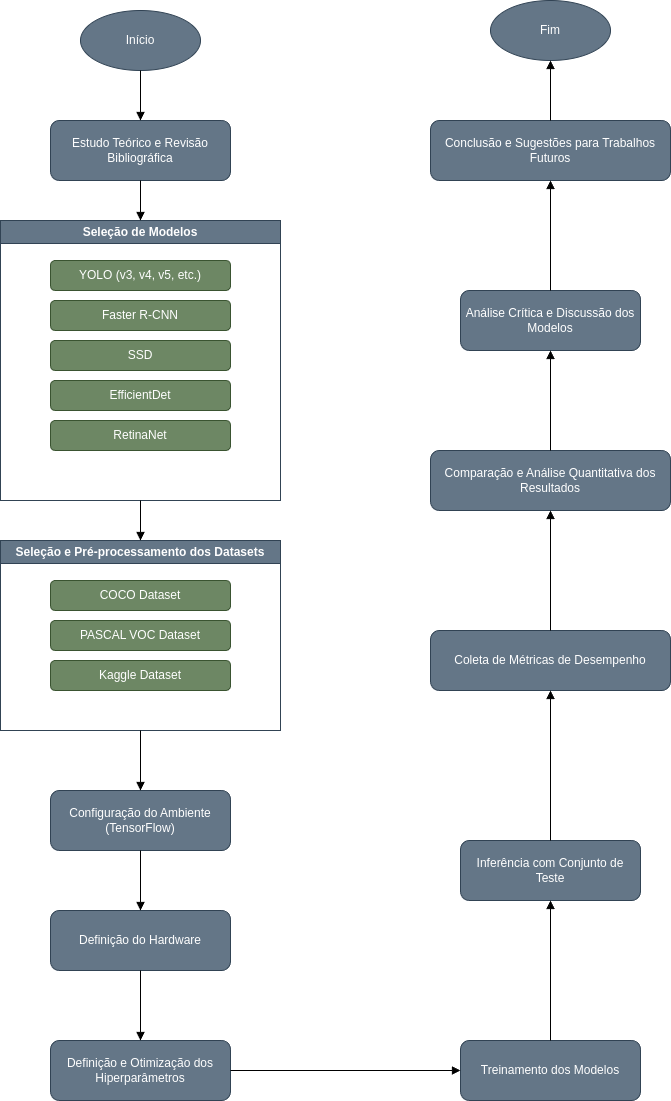
\includegraphics[width=0.8\textwidth]{media/fluxograma.png}
\fonte{Elaborado pelo autor (2025)}
\label{fig:fluxograma}
\end{figure}

\section{Estudo Teórico e Revisão Bibliográfica}

Nesta etapa, será realizado um estudo aprofundado sobre os fundamentos da visão computacional e do aprendizado de máquina, com foco em redes neurais de aprendizagem profunda. Serão revisados os conceitos e as arquiteturas de detecção de objetos mais relevantes, como YOLO, Faster R-CNN, SSD, EfficientDet e RetinaNet. Esta fase buscará fundamentar teoricamente a pesquisa, compreendendo as características, vantagens e limitações de cada modelo.

\section{Seleção e Pré-processamento dos Datasets}

Serão selecionados e pré-processados os principais datasets de referência para detecção de objetos, como o COCO Dataset, PASCAL VOC Dataset e Kaggle Dataset. O pré-processamento envolverá a preparação e organização dos dados para o treinamento dos modelos.

\section{Configuração do Ambiente e Definição do Hardware}

A configuração do ambiente de desenvolvimento será feita utilizando o framework TensorFlow. O Google Colab, com runtime que utiliza placa de vídeo dedicada, será empregado para o treinamento dos modelos, devido à sua acessibilidade e capacidade de processamento. Serão definidos os requisitos de hardware, levando em consideração as necessidades computacionais de cada modelo para o treinamento e inferência.

\section{Definição e Otimização dos Hiperparâmetros}

Nesta etapa, serão definidos e otimizados os hiperparâmetros de cada modelo para garantir o melhor desempenho possível durante o treinamento. Este processo é crucial para ajustar os modelos aos datasets e ao hardware disponível.

\section{Treinamento e Inferência dos Modelos}

Os modelos de detecção de objetos serão treinados com os datasets pré-processados. Após o treinamento, a inferência será realizada em um conjunto de testes para avaliar o desempenho de cada modelo em dados não vistos.

\section{Coleta de Métricas e Análise de Resultados}

Serão coletadas métricas de desempenho, como precisão, recall, mean Average Precision (mAP) e tempo de inferência. Os resultados serão comparados e analisados quantitativamente para identificar o equilíbrio entre precisão e velocidade de cada arquitetura.

\section{Análise Crítica e Discussão dos Modelos}

Com base na análise quantitativa, será realizada uma discussão crítica sobre o desempenho de cada modelo. Esta etapa considerará não apenas as métricas, mas também a complexidade de implementação e a escalabilidade, fornecendo subsídios para a escolha do algoritmo mais adequado a cada contexto.

\section{Conclusão e Sugestões para Trabalhos Futuros}

Por fim, o trabalho apresentará uma conclusão sobre os resultados obtidos e as principais contribuições da pesquisa. Serão feitas sugestões para trabalhos futuros, explorando possíveis melhorias e novas direções para a área de detecção de objetos.

% \chapter{DESENVOLVIMENTO}
\label{cap:desenvolvimento}
Vestibulum ac arcu suscipit, consequat orci sit amet, maximus dolor. Vestibulum condimentum
nulla vitae fermentum venenatis. In sit amet tincidunt ex, quis molestie turpis. Proin eleifend
fringilla tincidunt. Curabitur pellentesque nisi in risus iaculis, in tristique odio maximus.
Donec condimentum massa a erat malesuada, ut lacinia elit maximus. Integer feugiat volutpat
luctus. Vestibulum commodo varius venenatis. Ut diam ante, feugiat non consectetur id, suscipit
at dolor. Duis tempor quam ligula, id volutpat ligula dapibus id. Phasellus at fermentum nibh.

\section{Levantamento das Estórias}

As estórias foram identificadas, analisadas e descritas abaixo:

\begin{itemize}
	\item \textbf{Estória 01: Cadastrar Catador}\par
Descrição: Permite a criação do usuário responsável pelo recolhimento do material descartado.

	\item \textbf{Estória 02: Cadastrar Separador}\par
Descrição: Permite a criação do usuário responsável pelo descarte do material.

	\item \textbf{Estória 03: Efetuar login}\par
Descrição: Autoriza o acesso às funcionalidades do sistema. 

	\item \textbf{Estória 04: Recuperar senha }\par
Descrição: Possibilita que o usuário redefina a senha.

	\item \textbf{Estória 05: Tirar dúvidas }\par
Descrição: Esclarece sobre a definição dos perfis. 

	\item \textbf{Estória 06: Solicitar recolhimento}\par
Descrição: Requisita a coleta do material descartado.

	\item \textbf{Estória 07: Realizar logoff}\par
Descrição: Permite que o usuário saia do sistema.

\end{itemize}


\section{Diagramas do Modelo Proposto}

\subsection{Diagrama de Classes}

Na construção do diagrama de classes foi analisada as principais classes do sistema, suas
características, seus relacionamentos e suas funcionalidades. É possível observar através da
\autoref{fig:classe}, a estrutura do desenvolvimento do sistema.

%%%%%%%%%%%%%%%%%%%% Figure/Image No: 8 starts here %%%%%%%%%%%%%%%%%%%%

\begin{figure}[H]
	\caption{Diagrama de Classes}
	\begin{Center}
		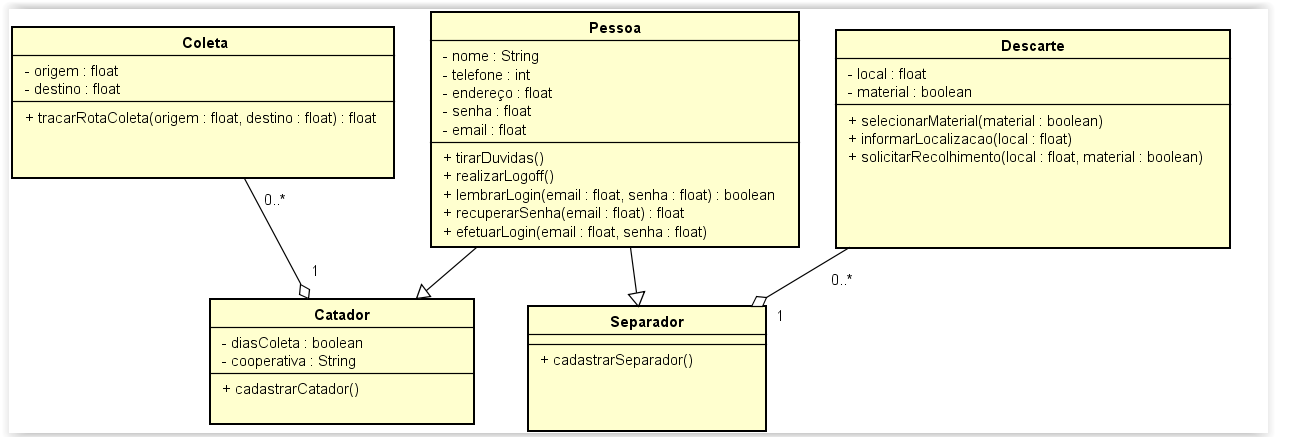
\includegraphics[width=6.4in,height=2.77in]{./media/image35.png}
	\end{Center}
	\label{fig:classe}
\end{figure}

%%%%%%%%%%%%%%%%%%%% Figure/Image No: 8 Ends here %%%%%%%%%%%%%%%%%%%%

Na \autoref{fig:classe} citada acima podemos observar o Diagrama de Classes utilizado para a
construção do aplicativo.

As classes Catador e Separador são extensões da classe Pessoa, que tem como objetivo informar
seus dados, tirar dúvidas sobre a definição dos perfis, criar uma conta perfil, redefinir a
senha esquecida, efetuar \textit{login}, salvar os dados do \textit{login} e realizar
\textit{logoff}.

A classe Catador que faz parte de uma das contas perfil, é responsável pelo cadastro do usuário
catador. Este usuário é encarregado por traçar a rota da coleta e recolher o material
descartado.

A classe Separador que faz parte de uma das contas perfil, é responsável pelo cadastro do
usuário separador. Ao informar sua localização e o tipo de material, o usuário poderá solicitar
o recolhimento do material descartado.

\subsection{Diagrama de Casos de Uso}

Esse parágrafo descreve as funcionalidades do sistema e as interações entre os atores, através
da \autoref{fig:casos}.

%%%%%%%%%%%%%%%%%%%% Figure/Image No: 9 starts here %%%%%%%%%%%%%%%%%%%%

\begin{figure}[H]
\caption{Diagrama de Casos de Uso}
	\begin{Center}
		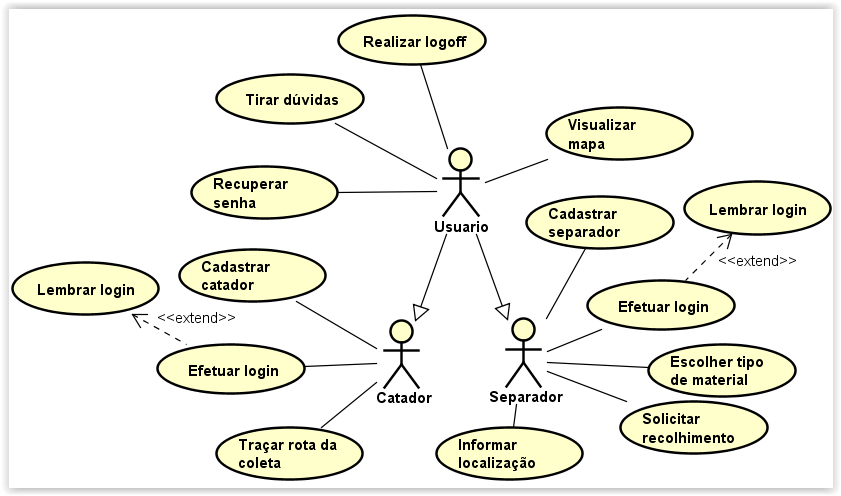
\includegraphics[width=5.12in,height=3.02in]{./media/image32.png}
	\end{Center}
	\label{fig:casos}
\end{figure}

%%%%%%%%%%%%%%%%%%%% Figure/Image No: 9 Ends here %%%%%%%%%%%%%%%%%%%%

Na \autoref{fig:casos} citada acima, podemos ver o Diagrama de Casos de Uso. Na tela inicial
do aplicativo, o usuário poderá realizar as seguintes funções: logar no APP, cadastrar usuário,
tirar dúvidas, efetuar \textit{logoff} e recuperar a senha. Se o usuário ainda não estiver
cadastrado, irá se cadastrar no perfil desejado: Catador ou Separador. Caso já tenha cadastro,
basta efetuar o \textit{login}, o qual pode ser salvo pelo sistema. Em caso de senha esquecida,
o sistema permite a recuperação através do \textit{e-mail}.

A partir da inserção da localização e do tipo de material, o Separador poderá solicitar o
recolhimento do rejeito. O Catador recebendo a solicitação do Separador, irá traçar a rota
para a coleta do material.

\paragraph*{5.2.2.1 Especificação dos Casos de Uso}

Esse capítulo é responsável pelo detalhamento das funcionalidades do sistema. O
(\autoref{quad:catador}), descreve o passo a passo para o cadastro do usuário Catador.

%%%%%%%%%%%%%%%%%%%% Table No: 4 starts here %%%%%%%%%%%%%%%%%%%%

\begin{quadro}[H]
\caption{Cadastrar Catador}
\label{quad:catador}
\centering
\begin{tabular}{p{1.25in}p{4.50in}}
\hline
%row no:1
\multicolumn{1}{|p{1.25in}}{\textbf{Caso de Uso}} & 
\multicolumn{1}{|p{4.50in}|}{Cadastrar Catador} \\
\hhline{--}
%row no:2
\multicolumn{1}{|p{1.25in}}{\textbf{Descrição}} & 
\multicolumn{1}{|p{4.50in}|}{Permite a criação de perfil usuário denominado catador.} \\
\hhline{--}
%row no:3
\multicolumn{1}{|p{1.25in}}{\textbf{Ator}} & 
\multicolumn{1}{|p{4.50in}|}{Catador} \\
\hhline{--}
%row no:4
\multicolumn{1}{|p{1.25in}}{\textbf{Pré-condições}} & 
\multicolumn{1}{|p{4.50in}|}{Preencher todos os dados solicitados} \\
\hhline{--}
%row no:5
\multicolumn{1}{|p{1.25in}}{\textbf{Pós-condições}} & 
\multicolumn{1}{|p{4.50in}|}{Cadastro do perfil catador no sistema} \\
\hhline{--}
%row no:6
\multicolumn{1}{|p{1.25in}}{\textbf{Fluxo Principal}} & 
\multicolumn{1}{|p{4.50in}|}{\begin{enumerate}[label*={\fontsize{12pt}{12pt}\selectfont \arabic*.}]
	\item Na tela inicial, o usuário solicita o cadastro; \par 	\item Em seguida preenche todos os dados; \par 	\item O sistema valida os dados preenchidos; \par 	\item O cadastro é realizado.
\end{enumerate}} \\
\hhline{--}
%row no:7
\multicolumn{1}{|p{1.25in}}{\textbf{Fluxo de Exceção}} & 
\multicolumn{1}{|p{4.50in}|}{\textbf{Dados incorretos} \par \begin{enumerate}[label*={\fontsize{12pt}{12pt}\selectfont \arabic*.}]
	\item No passo 3 do Fluxo Principal, o usuário não preencheu os dados corretamente, o sistema sinaliza qual campo não foi preenchido.
\end{enumerate} \par \textbf{Dados não cadastrados} \par \begin{enumerate}[label*={\fontsize{12pt}{12pt}\selectfont \arabic*.}]
	\item No passo 3 do Fluxo Principal, o usuário preenche algum campo já cadastrado, o sistema exibe qual campo já foi cadastrado.
\end{enumerate}} \\
\hhline{--}

\end{tabular}
\end{quadro}


%%%%%%%%%%%%%%%%%%%% Table No: 4 ends here %%%%%%%%%%%%%%%%%%%%

O caso de uso Cadastrar Catador (\autoref{quad:catador}), citado acima é responsável por
avaliar as ações necessárias para realizar o cadastro do perfil catador.

O \autoref{qua:separador} descreve o passo a passo para o cadastro do usuário Separador.

%%%%%%%%%%%%%%%%%%%% Table No: 5 starts here %%%%%%%%%%%%%%%%%%%%


\begin{quadro}[H]
\caption{Cadastro Separador}
 \label{qua:separador}		\begin{tabular}{p{1.33in}p{3.96in}}
\hline
%row no:1
\multicolumn{1}{|p{1.33in}}{\textbf{Caso de Uso}} & 
\multicolumn{1}{|p{3.96in}|}{Cadastrar Separador} \\
\hhline{--}
%row no:2
\multicolumn{1}{|p{1.33in}}{\textbf{Descrição}} & 
\multicolumn{1}{|p{3.96in}|}{Permite a criação de perfil usuário denominado separador.} \\
\hhline{--}
%row no:3
\multicolumn{1}{|p{1.33in}}{\textbf{Ator}} & 
\multicolumn{1}{|p{3.96in}|}{Separador} \\
\hhline{--}
%row no:4
\multicolumn{1}{|p{1.33in}}{\textbf{Pré-condições}} & 
\multicolumn{1}{|p{3.96in}|}{Preencher todos os dados solicitados } \\
\hhline{--}
%row no:5
\multicolumn{1}{|p{1.33in}}{\textbf{Pós-condições}} & 
\multicolumn{1}{|p{3.96in}|}{Cadastro do perfil separador no sistema} \\
\hhline{--}
%row no:6
\multicolumn{1}{|p{1.33in}}{\textbf{Fluxo Principal}} & 
\multicolumn{1}{|p{3.96in}|}{\begin{enumerate}[label*={\fontsize{12pt}{12pt}\selectfont \arabic*.}]
	\item Na tela inicial, o usuário solicita o cadastro; \par 	\item Em seguida, preenche todos os dados; \par 	\item O sistema verifica os dados; \par 	\item O cadastro é realizado.
\end{enumerate}} \\
\hhline{--}

\end{tabular}
 \end{quadro}

%%%%%%%%%%%%%%%%%%%% Table No: 5 ends here %%%%%%%%%%%%%%%%%%%%

O caso de uso Cadastrar Separador (\autoref{qua:separador}), citado acima é responsável por
avaliar as ações necessárias para realizar o cadastro do perfil separador.





% \chapter{RESULTADOS E DISCUSSÕES}
\label{cap:resultados}

\section{Desempenho Geral de Detecção}
\label{sec:desempenho-geral}

\section[O Dilema Precisão vs. Recall]{O Dilema Precisão \textit{vs.} Recall}
\label{sec:dilema-precisao-recall}

\section[O Impacto do Transfer Learning na Convergência]{O Impacto do Transfer Learning na Convergência}
\label{sec:impacto-transfer}

\section[O Efeito do Tamanho do Lote (Batch Size)]{O Efeito do Tamanho do Lote (\textit{Batch Size})}
\label{sec:batch-size}

\section[Limitações de Hardware e Tempos de Inferência]{Limitações de Hardware e Tempos de Inferência}
\label{sec:hardware-inferencia}

\section[Análise de Custo-Benefício Computacional]{Análise de Custo-Benefício Computacional}
\label{sec:custo-beneficio}

% \chapter{CONCLUSÃO}
\label{cap:conclusao}

\section{Síntese do Estudo}
\label{sec:sintese}

\section{Trabalhos Futuros}
\label{sec:trabalhos-futuros}

\glsaddall

\postextual

% Example citation (remove or replace with your actual citation)
\cite{exemplo-referencia}

\bibliographystyle{plain}
\bibliography{Referencias}

% Imprime uma página indicando o início dos apêndices
% \partapendices
\part*{Apêndices}

\begin{apendicesenv}


\chapter{Questionário de Avaliação do Protótipo}

\begin{figure}[H]
	\begin{Center}
		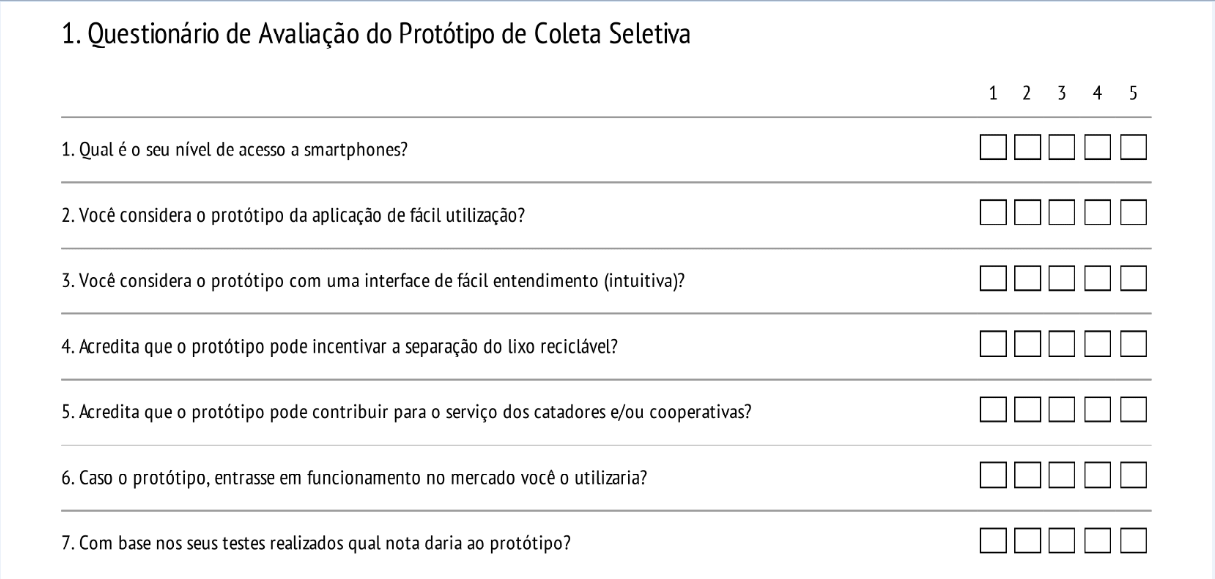
\includegraphics[width=6.00in]{media/questionariopaint.png}
		\label{fig:questionario}
	\end{Center}
\end{figure}

\chapter{Códigos fonte comentados}

\section{Salvar usuário catador no banco de dados}

O \autoref{cod:cadbanc} é responsável por salvar o usuário catador no \textit{firebase realtime database}. A linha 3 do \autoref{cod:cadbanc}, consiste na criação do nó (\textit{child}) denominado “Catadores”, onde cada catador possui um identificador (\textit{id}), onde seus dados são salvos (\textit{setValue}).

\begin{codigo}[H]
\begin{lstlisting}[language=Java]
public void salvar(){
    DatabaseReference databaseReference = ConfiguracaoFirebase.getFirebase();
    databaseReference.child("Catadores").child(getId()).setValue(this);
}
\end{lstlisting}
\caption{Salvar usuário catador no banco de dados}
\label{cod:cadbanc}
\end{codigo}


\section{Salvar usuário separador no banco de dados}

\begin{codigo}[H]
	\begin{lstlisting}[language=Java]
public void salvar(){
    DatabaseReference databaseReference = ConfiguracaoFirebase.getFirebase();
    databaseReference.child("Separadores").child(getId()).setValue(this);
}
   	\end{lstlisting}
   	\caption{Salvar usuário separador no banco de dados}
   	\label{cod:cadsep}
\end{codigo}

O \autoref{cod:cadsep} é responsável por salvar o usuário separador no \textit{firebase realtime database}. A linha 3 do \autoref{cod:cadbanc}, consiste na criação do nó (\textit{child}) denominado “Separadores”, onde cada separador possui um identificador (\textit{id}), onde seus dados são salvos (\textit{setValue}).


\section{Cadastrar usuário catador}

\begin{codigo}[H]
	\begin{lstlisting}[language=Java]
private void cadastrarCatador(){
    firebaseAuth = ConfiguracaoFirebase.getFirebaseAuth();
    firebaseAuth.createUserWithEmailAndPassword(
            catador.getEmail(),
            catador.getSenha()
    ).addOnCompleteListener(CadastroCatador.this, new OnCompleteListener<AuthResult>() {
        @Override
        public void onComplete(@NonNull Task<AuthResult> task) {
            if(task.isSuccessful()){
                Toast.makeText(CadastroCatador.this,"Sucesso ao cadastrar catador",Toast.LENGTH_LONG).show();
                FirebaseUser firebaseUser = task.getResult().getUser();
                catador.setId(firebaseUser.getUid());
                catador.salvar();
                startActivity(new Intent(CadastroCatador.this, Login.class));
       	\end{lstlisting}
       	\caption{Cadastrar usuário catador na aplicação}
       	\label{cod:cat}
\end{codigo}

O \autoref{cod:cat} consiste no cadastro do usuário catador. A função \textit{createUserWithEmailAndPassword}, que se encontra na linha 3, é responsável pela criação da autenticação dos usuário através do \textit{e-mail} e a senha. Em caso de sucesso, o sistema irá exibir a seguinte mensagem “Sucesso ao cadastrar catador” e o usuário será redirecionado para a tela de \textit{login}.

\section{Cadastrar usuário separador}

\begin{codigo}[H]
	\begin{lstlisting}[language=Java]
private void cadastrarSeparador(){
    firebaseAuth = ConfiguracaoFirebase.getFirebaseAuth();
    firebaseAuth.createUserWithEmailAndPassword(
            separador.getEmail(),
            separador.getSenha()
    ).addOnCompleteListener(CadastroSeparador.this, new OnCompleteListener<AuthResult>() {
        @Override
        public void onComplete(@NonNull Task<AuthResult> task) {
            if(task.isSuccessful()){
                Toast.makeText(CadastroSeparador.this,"Sucesso ao cadastrar separador",Toast.LENGTH_LONG).show();
                FirebaseUser firebaseUser = task.getResult().getUser();
                separador.setId(firebaseUser.getUid());
                separador.salvar();
                startActivity(new Intent(CadastroSeparador.this, Login.class));
       	\end{lstlisting}
       	\caption{Cadastrar usuário separador}
       	\label{cod:sep}
\end{codigo}

O \autoref{cod:sep} consiste no cadastro do usuário separador. A função \textit{createUserWithEmailAndPassword}, que se encontra na linha 3, é responsável pela criação da autenticação do usuário através do \textit{e-mail} e a senha.

\end{apendicesenv}

\begin{anexosenv}




\end{anexosenv}

\end{document}
